\documentclass[10pt,a4paper]{article}
\usepackage[margin=2.1cm]{geometry}
\usepackage[T1]{fontenc}
\usepackage{lmodern}
\usepackage{amsmath,amssymb}
\usepackage{graphicx}
\usepackage{booktabs}
\usepackage{xcolor}
\usepackage{listings}
\usepackage{enumitem}
\usepackage[hidelinks]{hyperref}
\usepackage{caption}
\captionsetup{font=small,labelfont=bf}
\setlist{itemsep=2pt,topsep=3pt}
\definecolor{boxbg}{HTML}{EEF4FC}
\definecolor{codebg}{HTML}{F6F6F4}
\lstset{language=Python,basicstyle=\ttfamily\footnotesize,backgroundcolor=\color{codebg},
        frame=none,columns=fullflexible,keepspaces=true,showstringspaces=false,
        xleftmargin=4pt,aboveskip=4pt,belowskip=4pt}

\title{\vspace{-1.2cm}Larger initial overlaps for the log-balanced study\\[2pt]
\large same Hamiltonians, different initial states}
\date{19 October 2026}
\author{}

\begin{document}
\maketitle
\vspace{-1.4cm}

\noindent\colorbox{boxbg}{\parbox{\dimexpr\linewidth-2\fboxsep}{%
\textbf{In short}
\begin{enumerate}[leftmargin=1.4em]
\item \textbf{The small overlaps come from how the initial states are drawn, not from the
  Hamiltonians.} The study draws them uniformly from every basis state with $p>10^{-12}$.
  Most of those states lie in the exponentially small tail of the ground state, so the
  median overlap is $10^{-6.6}$ and 55\% of the runs start below $10^{-6}$.
\item \textbf{The current overlap is tangled with the density} (correlation 0.59 between
  $\log_{10}$ overlap and $\log_{10}$ density). A low-density ground state has a few heavy
  states and a huge light tail, and the uniform draw lands in the tail. The ``by overlap''
  plots are therefore partly ``by density'' plots.
\item \textbf{Recommendation:} draw the initial states uniformly from the states the density
  counts, $p>0.1/2^N$. This is a one-line change in \texttt{run\_cell}. The median overlap
  rises to $10^{-2.7}$, no run starts below $0.1/2^N$, and the overlap becomes independent
  of the density (correlation $-0.07$). The Hamiltonians are unchanged.
\item \textbf{The price:} a ground state with fewer than six such states gets fewer initial
  states. This affects 715 of the 2880 Hamiltonians, all with density below $10^{-1.1}$, and
  gives 14\,491 instead of 17\,280 runs. The dropped runs are exactly the ones that started
  around $10^{-9}$.
\end{enumerate}}}

\section*{1\quad Where the overlaps come from}
I used the 2880 Hamiltonians the production run selected (\texttt{balanced\_hamiltonians\_log.csv}
in the shard directory): 20 per $(N,\text{dimension},\Delta,\text{max distance})$. I solved
every ground state once and drew six initial states per Hamiltonian under several schemes
(\texttt{initial\_states.py}). The scheme \emph{current} uses the same generator and the same
call as \texttt{run\_cell}. It reproduces 17\,274 of the 17\,280 production runs state by state,
so the numbers below describe the data in the shards.

The current draw spreads the overlap almost evenly in $\log_{10}$ from $10^{-12}$ up to about
$10^{-3}$ (Fig.~\ref{fig:schemes}, top row). The ground state has some weight on nearly every
basis state of its symmetry sector, but almost all of that weight sits on a few of them. The
remaining states fill the decades below. A uniform pick from the support is therefore almost
always a tail state.

Fig.~\ref{fig:density} (top row) shows the consequence. The lower the density, the more tail
there is to draw from. At $\log_{10}$ density $<-2$, 86\% of the initial states start below
$10^{-6}$, although the same Hamiltonians offer states with $p\approx1$ (grey).

\section*{2\quad Alternatives}
All schemes keep the Hamiltonians and change only which six basis states are started from.

\begin{table}[h]
\centering\footnotesize\setlength{\tabcolsep}{4.5pt}
\begin{tabular}{lrrrrrrrr}
\toprule
scheme & runs & $q_{5}$ & median & $q_{95}$ & $>10^{-2}$ & $>10^{-3}$ & $<10^{-6}$ & corr.\\
\midrule
current: uniform, $p>10^{-12}$ & 17\,280 & $-11.4$ & $-6.6$ & $-1.8$ & 6\% & 15\% & 55\% & 0.59\\
\textbf{dense: uniform, $p>0.1/2^N$} & \textbf{14\,491} & $\mathbf{-4.4}$ & $\mathbf{-2.7}$ & $\mathbf{-0.0}$ & \textbf{29\%} & \textbf{61\%} & \textbf{0\%} & $\mathbf{-0.07}$\\
dense, topped up to six & 17\,280 & $-9.9$ & $-2.9$ & $-0.1$ & 25\% & 51\% & 13\% & 0.44\\
stratified in $\log_{10}p$ & 16\,019 & $-11.0$ & $-4.8$ & $-0.0$ & 17\% & 28\% & 39\% & 0.15\\
stratified in $\log_{10}p$, $p>0.1/2^N$ & 10\,690 & $-4.0$ & $-2.2$ & $-0.0$ & 45\% & 75\% & 0\% & $-0.28$\\
with probability $p$ (Born) & 17\,280 & $-4.7$ & $-2.1$ & $-0.0$ & 47\% & 73\% & 1\% & 0.38\\
\midrule
the six largest $p$ (reference) & 17\,280 & $-4.6$ & $-1.7$ & $-0.0$ & 61\% & 79\% & 1\% & 0.51\\
\bottomrule
\end{tabular}
\caption{Initial overlaps of the 2880 selected Hamiltonians, six initial states each.
$q_5$, median and $q_{95}$ are quantiles of $\log_{10}$ overlap. The last column is the
correlation of $\log_{10}$ overlap with $\log_{10}$ density over all runs.}
\label{tab:schemes}
\end{table}

\begin{description}[leftmargin=0pt,style=unboxed]
\item[Dense (recommended).] It removes the tail and nothing else. The overlap then lies between
  $0.1/2^N$ and the largest $p$ of the Hamiltonian, and it no longer depends on the density.
  It uses the same threshold as the density, so ``the ground state'' means the same set of
  states in both quantities.
\item[Dense, topped up.] It keeps six runs per Hamiltonian, but the top-up states of the
  low-density Hamiltonians come from the tail again. That brings back 13\% of runs below
  $10^{-6}$ and the correlation with the density (0.44).
\item[Stratified.] It covers the whole range, $10^{-11}$ to 1, evenly per Hamiltonian, but
  still puts 39\% of the runs below $10^{-6}$. Use it only if the tiny overlaps are wanted
  for their own sake. Restricted to $p>0.1/2^N$, it leaves too few runs, since strata stay
  empty.
\item[Born.] Drawing with probability $p$ is what measuring the ground state would return,
  and it gives the largest typical overlaps. It is still correlated with the density (0.38):
  after the heavy states of a low-density Hamiltonian are taken, the draw without replacement
  falls into the tail.
\end{description}

\begin{figure}[t]
\centering
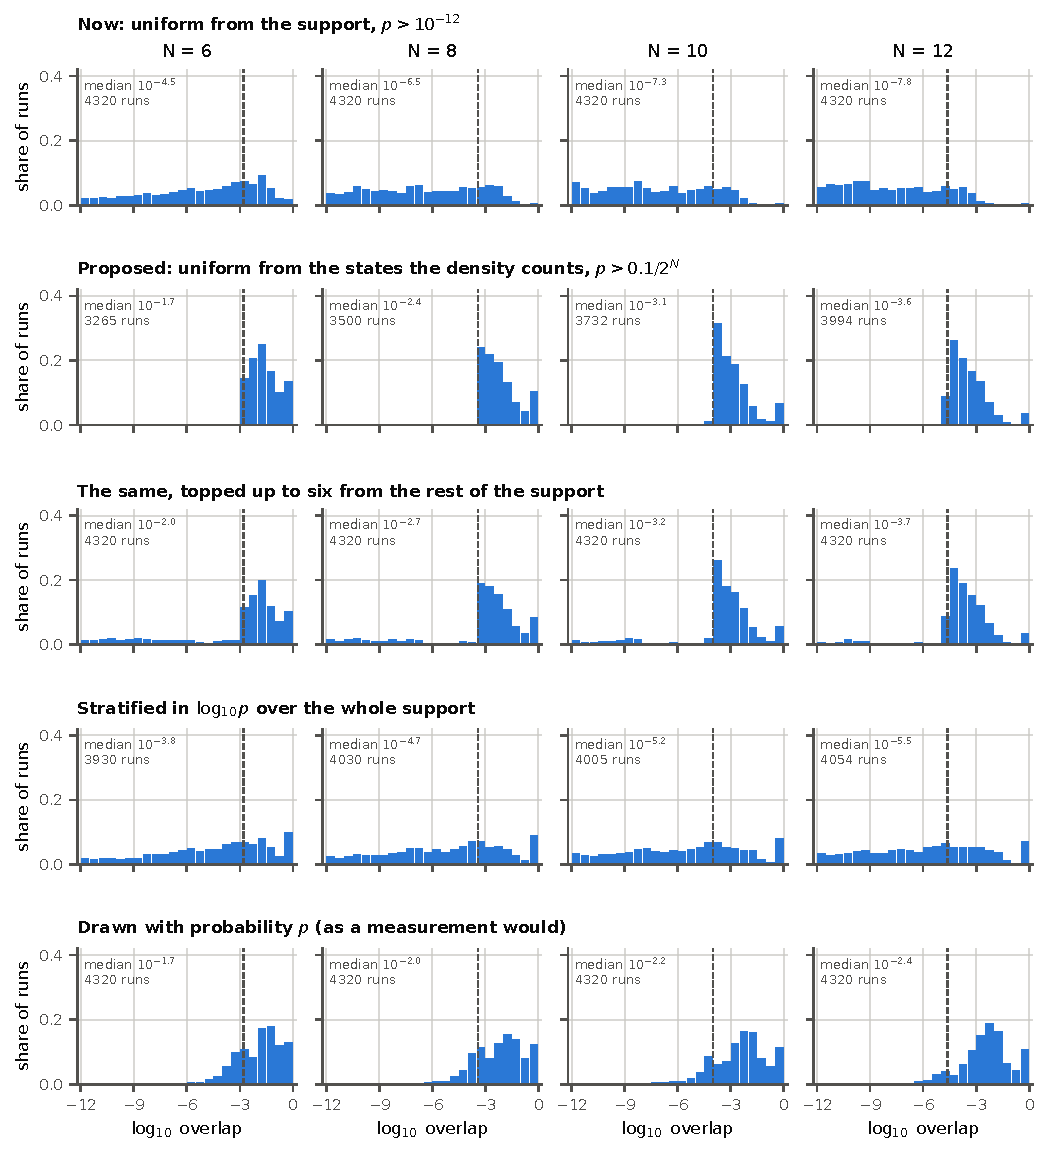
\includegraphics[width=\linewidth]{figures/overlap_schemes.pdf}
\caption{Distribution of the initial overlap per scheme (rows) and system size (columns),
over all selected Hamiltonians. The dashed line is $0.1/2^N$, the threshold of the density.}
\label{fig:schemes}
\end{figure}

\begin{figure}[t]
\centering
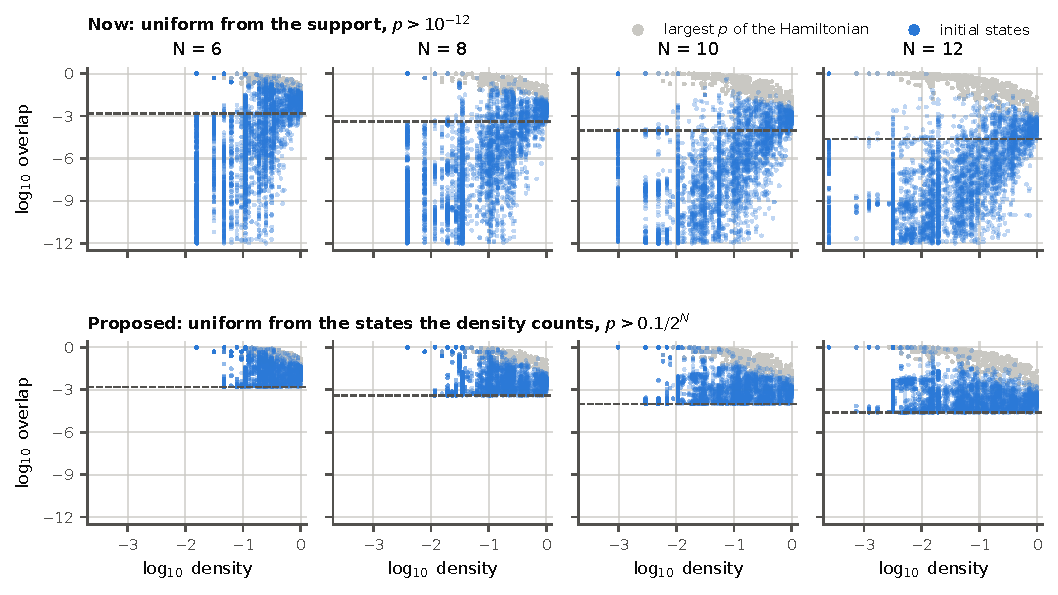
\includegraphics[width=\linewidth]{figures/overlap_vs_density.pdf}
\caption{Initial overlap against ground-state density, now and with the recommended draw.
Grey: the largest $p$ of each Hamiltonian, i.e.\ the largest overlap it can offer at all. The
dashed line is $0.1/2^N$.}
\label{fig:density}
\end{figure}

\section*{3\quad What sets the range}
With the recommended draw, the overlap of a run lies between $0.1/2^N$ and the largest $p$ of
its Hamiltonian (Fig.~\ref{fig:density}, bottom row). Both bounds are physical, so no draw can
move them.
\begin{itemize}
\item \textbf{The lower bound falls with $N$}, from $10^{-2.8}$ at $N=6$ to $10^{-4.6}$ at
  $N=12$, and the median follows it: $10^{-1.7}$, $10^{-2.4}$, $10^{-3.1}$ and $10^{-3.6}$ at
  $N=6,8,10,12$. A dense ground state at $N=12$ spreads its weight over thousands of states,
  so each of them carries about $1/2^N$. If overlaps should be compared across $N$, the
  relative overlap $p\cdot2^N$ is the natural axis.
\item \textbf{The upper bound falls with the density}, because a dense ground state has no
  heavy state. Three quarters of the overlaps above $10^{-1}$ come from Hamiltonians with
  density below $10^{-1}$.
\end{itemize}

\section*{4\quad How to change it}
In \texttt{EqualNumberOfBitstrings.run\_cell}, draw from the states the density counts:
\begin{lstlisting}
# before
non_zero_indices = np.flatnonzero(probabilities > OVERLAP_FLOOR)
# after: the states the ground-state density counts, p > 0.1 / 2^N
non_zero_indices = np.flatnonzero(probabilities > 0.1 / probabilities.size)
\end{lstlisting}
Everything else can stay.
\begin{itemize}
\item The Hamiltonians, the per-cell seeds and with them the SKQD shots are unchanged.
\item \texttt{load\_partial} and \texttt{merge} already accept cells with fewer than
  \texttt{num\_initial\_states} initial states. A cell is checked in blocks of one initial
  state, so these cells count as finished rather than being redone.
\item The run needs a new \texttt{SHARD\_DIR}. Copy \texttt{balanced\_hamiltonians\_log.csv}
  into it first: then plan reads the Hamiltonians instead of selecting them again, and they
  are guaranteed to be the same ones.
\item There are 16\% fewer runs, so the array finishes sooner.
\end{itemize}

\vspace{4pt}
\noindent\small Reproduce in \texttt{StudyOfHamiltonians/}: \texttt{python initial\_states.py},
then \texttt{python overlap\_figures.py}, then \texttt{pdflatex overlap\_report.tex}.
\end{document}
